\documentclass[xcolor=dvipsnames,aspectratio=169]{beamer}

% Standard packages
\usepackage{amsmath,amsthm,amsfonts,mathabx}
\usepackage{babel}
\usepackage[utf8]{inputenc}
\usepackage[T1]{fontenc}
\usepackage{graphicx}
\usepackage{listings}

% Basic Julia definition for lstlisting
\input juliadef.tex

\lstdefinelanguage{LDRjl}{
  language=Julia,
  morekeywords=[2]{LinearDecisionRules,LDRModel,Uncertainty,SolvePrimal,SolveDual,get_decision,FirstStage,BreakPoints,set_parametric_objective},
  keywordstyle=[2]\bfseries\color{red},
}

\definecolor{mygreen}{RGB}{34,139,34}
\lstset{%
    language         = LDRjl,
    basicstyle       = \ttfamily,
    keywordstyle     = \bfseries\color{blue},
    stringstyle      = \color{magenta},
    commentstyle     = \color{mygreen},
    showstringspaces = false,
    breaklines       = true,
    extendedchars    = true,
    literate={≈}{{$\approx$}}1%
}

% Setup appearance and colors
\usetheme{Boadilla}
\setbeamertemplate{page number in head/foot}[appendixframenumber]

\setbeamercovered{invisible}
\usefonttheme[onlymath]{serif}
\setbeamertemplate{enumerate items}[default]
\definecolor{mpl-c2}{HTML}{2ca02c}

\setbeamercolor{emph}{fg=blue}
\renewcommand<>{\emph}[1]{%
  {\usebeamercolor[fg]{emph}\only#2{\itshape}#1}%
}

\newcommand<>{\blue}[1]{{\only#2{\color{blue}}#1}}
\newcommand<>{\alertt}[1]{\alert#2{\texttt{#1}}}

% Commands
\DeclareMathOperator{\Tr}{Tr}


% General structure
% 1) From LDR to LFDR
% Feedback control leads to product of variables
% A further approximation allows to separate
% Piecewise linear feedback for a bit more flexibility => needs convexification, but is ok for primal
% 2) Generalizations
% Can choose other basis for the uncertainties as well
% Dual decision rules are not lower bounds
% Dual recursion could be employed, links to DualSDDP
% 3) Examples
% 4) Open questions
% How to estimate P(x_t); LFDR is a ``scalarization'' for \min_\Pi V_{LFDR}(\Pi)

\begin{document}

\title[LDR + VF]
      {Value functions in \texttt{LinearDecisionRules.jl}}
\author[Bernardo Costa]
       {Bernardo Freitas Paulo da Costa (FGV)\\[2ex]
       with Joaquim Garcia (PSR)}
\date[ICSP 2025]{ICSP 2025, Paris}

% Multiple logos
\titlegraphic{
  \vskip -2cm
  \hspace{10cm}
  \uncover<2>{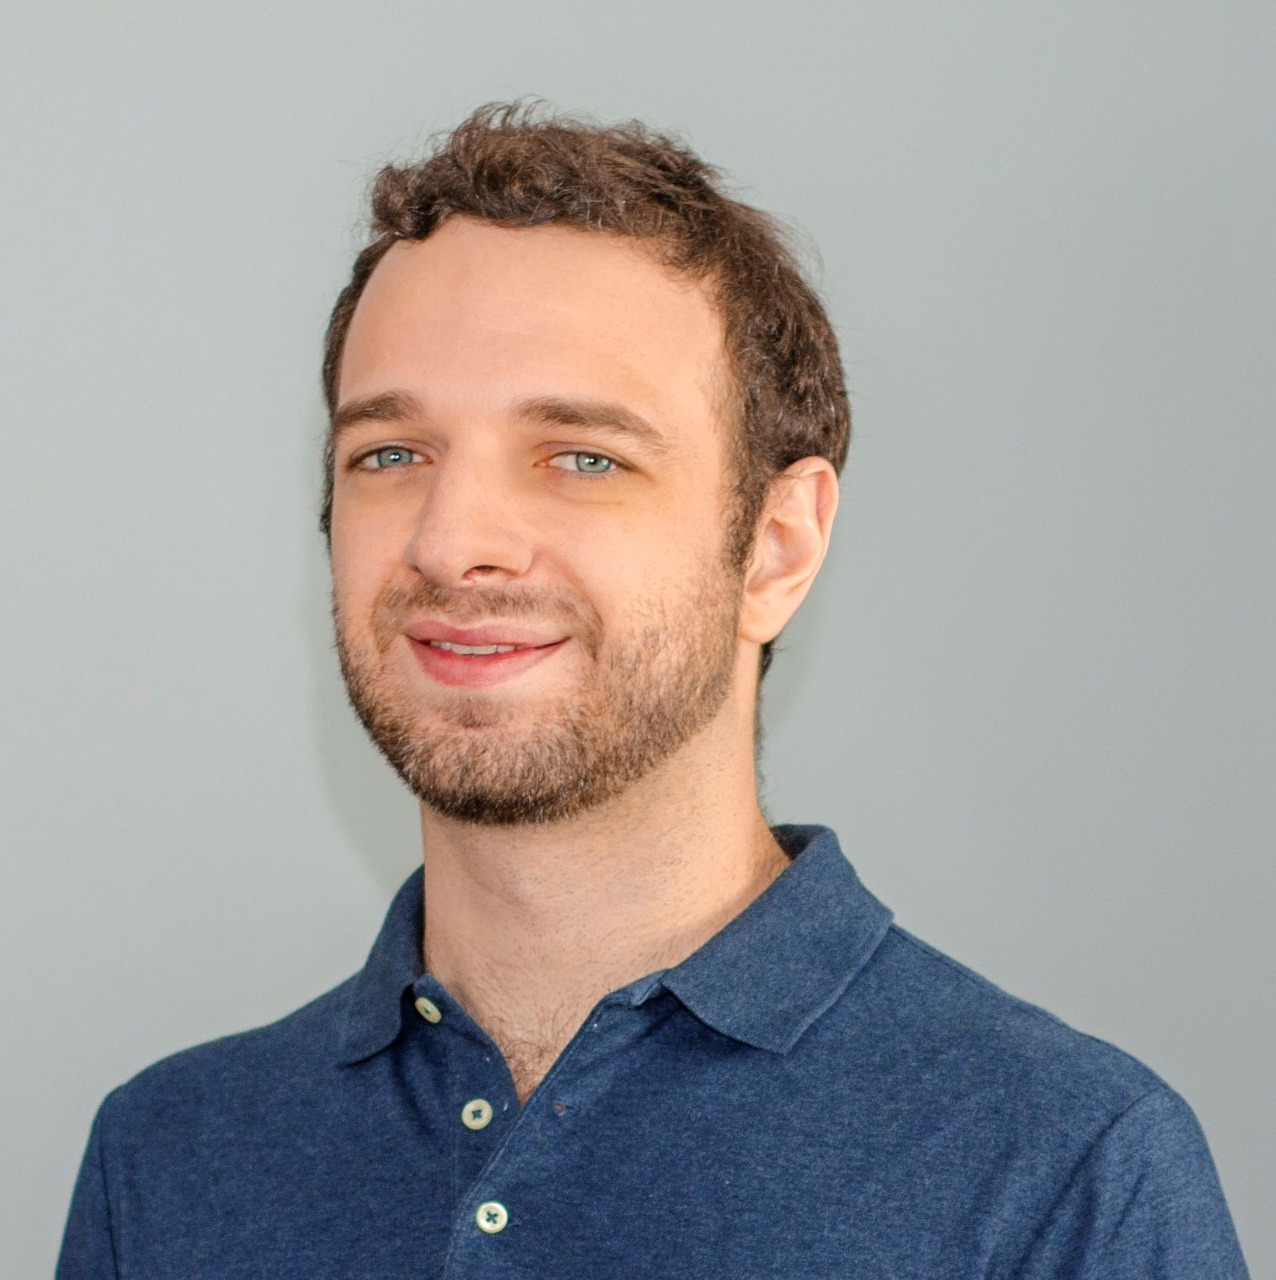
\includegraphics[width=3.5cm]{figures/Joaquim.jpeg}}
}

\begin{frame}
\titlepage
\end{frame}

\section{Introduction}

\subsection{Setting}

\begin{frame}{2-Stage Stochastic Programming}
  Basic model:
  \[ \begin{array}{rll}
    \min        & & \blue<2->{\mathbb{E}\left[ c(\xi)^\top y(\xi) \right]} \\[0.5ex]
    \text{s.t.} & A x = b, & \blue<2->{T x + W y(\xi) = h(\xi)} \\
    & x \geq 0, & \blue<2->{y(\xi) \geq 0},
  \end{array} \]
  \begin{itemize}
    \item $x$ is here-and-now, \blue<2->{$y$ is wait-and-see};
    \item $c$ are \blue<2->{(possibly random)} costs.
  \end{itemize}
  \pause[2]
\end{frame}

\begin{frame}{2-Stage Stochastic Programming}{Linear Decision Rules}
  \begin{itemize}
    \item Fix a parametrization where $c(\xi) = C \xi$ and $h(\xi) = H \xi$ are \alert{linear} in $\xi$.
    \item Posit a \alert{linear decision rule}: \( y(\xi) = Y \cdot \xi \).
  \end{itemize}
  \pause\medskip

  Reduces the flexibility of the ``wait-and-see'' decision\uncover<3->{, but allows for a \emph{finite} problem if the support of $\xi$ is simple, say $\Xi = \{\,\xi \mid G\xi \geq f\,\}$.}
  \[ \begin{array}{rll}
    \min        & & \mathbb{E}\left[ \xi^\top C^\top Y \xi \right] \uncover<3->{\blue{{} = \Tr\left(\mathbb{E}\big[ \xi \xi^\top \big] C^\top Y \right)}}\\[0.5ex]
    \text{s.t.} & A x = b & \alt<3->{\blue{Tx + W Y = H}}{T x + W Y \xi = H \xi \quad \forall \xi} \\
    & x \geq 0 & \alt<3->{\blue{Y = \Lambda G, \ \Lambda \geq 0, \ \Lambda f \geq 0}}{Y \xi \geq 0},
  \end{array} \]
  \pause[4]

  The distribution of $\xi$ appears only in the objective function, and through the 2${}^\text{nd}$-moment matrix $\mathbb{E}\left[\xi \xi^\top \right]$.
\end{frame}

\begin{frame}{2-Stage Stochastic Programming}{Sample Average Approximation: SAA}
  Kelley's cutting plane / L-shaped method builds approximations to the \blue{value function}
  \[
    \blue{V(x)} = \begin{array}[t]{rl}
      \min\limits_{y(\xi)} & \mathbb{E} \left[ c(\xi)^\top y(\xi) \right] \\
      \text{s.t.} & W y(\xi) = h(\xi) - T x, \\
      & y(\xi) \geq 0.
    \end{array}
  \]
  \pause
  Key points:
  \begin{itemize}
    \item $V(x)$ is a \emph{convex function} of $x$, so $V(x) \geq V(x_0) + \nabla V(x_0)^\top (x - x_0)$ for any $x_0$;
    \item The gradient $\nabla V(x_0)$ is given by the \emph{optimal dual solution} of the SAA problem at $x_0$.
  \end{itemize}

  \pause
  Exchanging $\min$ and $\mathbb{E}$:
  \[
    V(x) = \mathbb{E}\left[ \min_{y \in Y(x, \xi)} c(\xi)^\top y(x, \xi) \right]
  \]
  shows that \emph{$y$ is a feedback control}: depends on the uncertainty $\xi$ and the 1${}^\text{st}$-stage decision $x$.
\end{frame}

\begin{frame}{Multistage problems}
  \begin{itemize}
    \item The 2-stage problem can be generalized to \emph{multistage} problems, where the uncertainty $\xi$ is observed at different stages: $\xi_1, \xi_2, \ldots, \xi_T$;
    \item The decision $y_t(\xi)$ at stage $t$ can depend on the uncertainty observed at previous stages.\pause
    \item Typically, there is a \emph{state} $x_t(\xi)$ at each stage, depending on the realization of the uncertainties and the decisions $y_t$. 
  \end{itemize}
  \pause\medskip

  A multistage problem can be written as:
  \[
    \begin{array}{rll}
      \min        & \mathbb{E}\left[ \sum_{t=1}^T c_t(\xi)^\top y_t(\xi) \right] \\[0.5ex]
      \text{s.t.} & A x_t(\xi) + B x_{t-1}(\xi) + W y_t(\xi) = h_t(\xi) \quad \forall t\\
      & x_t \geq 0, \ y_t(\xi) \geq 0.
    \end{array}
  \]
\end{frame}

\begin{frame}{Multistage problems}
  \begin{block}{Linear Decision Rules}
  \begin{itemize}
    \item The decision $x_t(\xi)$ can depend on the \emph{history} of the uncertainties $\xi_1, \ldots, \xi_t$;
    \item The LDR becomes $x_t(\xi) = X_{t,1} \cdot \xi_1 + X_{t,2} \cdot \xi_2 + \ldots + X_{t,t} \cdot \xi_t$.
    \pause
    \item \alert{Increases} the number of decision variables for the LDR matrices.
  \end{itemize}
  \end{block}
  \pause\medskip

  \begin{block}{SAA}
  \begin{itemize}
    \item We discretize the uncertainty process into a finite number of scenarios, organized into a scenario tree.
    \item There is a value function $V_n$ for each \emph{node} of the tree.
  \end{itemize}
\end{block}
  
\end{frame}

\begin{frame}{Multistage problems}{Stagewise independence}
  If the realization $\xi_t$ at stage $t$ is independent of the previous realizations $\xi_1, \ldots, \xi_{t-1}$, then the value functions depend \emph{only on the stage $t$}.
  \begin{itemize}
    \item Efficient \emph{dynamic programming} recursion, calculating $V_t(x_{t-1})$ from $V_{t+1}(x_t)$:
    \[
      V_t(x_{t-1}) = \min_{\text{feasible } x_t, y_t} \mathbb{E}_{\xi_t}\left[ c_t(\xi_t)^\top y_t(\xi_t) + V_{t+1}(x_t(\xi_t)) \right].
    \]
    \item One standard algorithm is \emph{SDDP}, exploring the state space using Monte Carlo sampling of scenarios (and building cuts).
  \end{itemize}
\end{frame}

\begin{frame}{Our goals}
  \begin{itemize}
    \item Build \emph{time decompositions} suitable for linear decision rules;
    \item Recover \emph{value functions} from such decompositions;
    \item Obtain a \emph{reasonable policy} with moderate computational effort.
  \end{itemize}
\end{frame}


\begin{frame}{Back to the 2-stage problem}
  Notation: $x$ is the incoming state, $y$ the decision, and $z$ the outgoing state:
  \[
    V(x) = \begin{array}[t]{rl}
      \min        & \mathbb{E}\left[ c(\xi)^\top y(x, \xi) + f(z(x, \xi)) \right] \\[0.5ex]
      \text{s.t.} & T x + W_y y(x, \xi) + W_z z(x, \xi) = h(\xi) \\
      & y(x, \xi), z(x, \xi) \geq 0.
    \end{array}
  \]
  \pause

  \begin{itemize}[<+->]
    \item Decisions $y$ (and $z$) depend on the previous state $x$ and the uncertainty $\xi$;
    \item The LDR for this problem sets $y(x,\xi) = Y_\xi(x) \cdot \xi$ and $z(x,\xi) = Z_\xi(x) \cdot \xi$;
    \item The Linear Feedback Decision Rule (LFDR) sets
    $\begin{cases}
      y(x,\xi) = Y_\xi \cdot \xi + Y_x \cdot x \quad \text{and} \\
      z(x,\xi) = Z_\xi \cdot \xi + Z_x \cdot x.
    \end{cases}$
  \end{itemize}
\end{frame}

\begin{frame}{Some observations}

  \begin{enumerate}[<+->]
    \item Several ``value function recursions'':
  \begin{align*}
    V(x) & = \mathbb{E}_{\xi} \left[ c(\xi)^\top y^*(\xi) + f(z^*(\xi)) \right] \\
    V_{LDR}(x) & = \mathbb{E}_{\xi} \left[ c(\xi)^\top Y^*(x) \cdot \xi + \alt<3->{\blue{F^*(x) \cdot \xi}}{f(Z^*(x) \cdot \xi)} \right] \\
    V_{LFDR}(x) & = \mathbb{E}_{\xi} \left[ c(\xi)^\top (Y_\xi \cdot \xi + Y_x \cdot x) + \alt<3->{\blue{F_\xi \cdot \xi + F_x \cdot x}}{f(Z_\xi \cdot \xi + Z_x \cdot x)} \right].
  \end{align*}
  
  \item For fixed $x$, the LFDR is a feasible LDR for both $y$ and $z$, so $V_{LFDR}(x) \geq V_{LDR}(x) \geq V(x)$.
  \medskip

  \item We also need to represent $f(z)$ as \blue{linear functions\ldots}
  \item So $\frac{\partial V_{LFDR}(x)}{\partial x}$ is constant!
  \end{enumerate}
\end{frame}

\begin{frame}{More general decision rules}
  
  \begin{itemize}
    \item We \emph{lift} $x$ to a higher-dimensional space and only require that the decision rule is linear in the \emph{lifted} variables;
    \item If $x = \sum_{i=1}^J x_i$, this leads to a piecewise-linear decision rule.
    \pause

    \item We have $V_{PWLF}(x) = \mathbb{E}\left[ c(\xi)^\top (\hat{Y}_\xi \cdot \xi + \hat{Y}_x \cdot \blue{L(x)}) + \ldots \right]$.
    \pause
    \item $L(x)$ is a \emph{piecewise-linear} function, so we might need to \emph{convexify} $V_{PWLF}$.
  \end{itemize}
  \pause
  \begin{theorem}
    The natural polyhedral representation, including the simplicial constraints
    \[ 0 \leq x_J \leq \cdots \leq x_2 \leq x_1 \leq (\max x)/J \]
    \pause
    yields \(
    \begin{cases}
      \text{a convexification of $V_{PWLF}$;} \\ \pause
      \text{which remains a valid upper bound for $V_{LDR}(x)$, so for $V(x)$.}
    \end{cases} \)
  \end{theorem}
\end{frame}


\begin{frame}[fragile]{A toy example}
  \small
  \begin{lstlisting}{language=LDRjl}
    using JuMP, LinearDecisionRules
    using Ipopt, Distributions

    demand = 0.3
    
    m = LDRModel(Ipopt.Optimizer)
    @variable(m, vi in Uncertainty(distribution=Uniform(0,1)))
    @variable(m, inflow in Uncertainty(distribution=Uniform(0,0.2)))
    @variable(m, 0 <= vf <= 1)
    @variable(m, gh >= 0.0)
    @variable(m, gt >= 0.0)

    @constraint(m, balance, vf == vi - gh + inflow)
    @constraint(m, gt + gh == demand)

    @objective(m, Min, gt^2 + vf^2/2 - vf + 0.5)
  \end{lstlisting}
\end{frame}

\begin{frame}[fragile]{A toy example (cont.)}
  \small
  \begin{lstlisting}{language=LDRjl}
    # Solve the primal LDR
    set_attribute(m, SolvePrimal(), true)
    set_attribute(m, SolveDual(), false)
    set_attribute(vi, BreakPoints(), 5)
    optimize!(m)

    # Get the value function
    VF = JuMP.Model()
    @variable(VF, x)
    @objective(VF, Min, 0.0)
    set_parametric_objective!(VF, m, Dict(vi => x))
  \end{lstlisting}
\end{frame}

\begin{frame}{A toy example}
  \centering 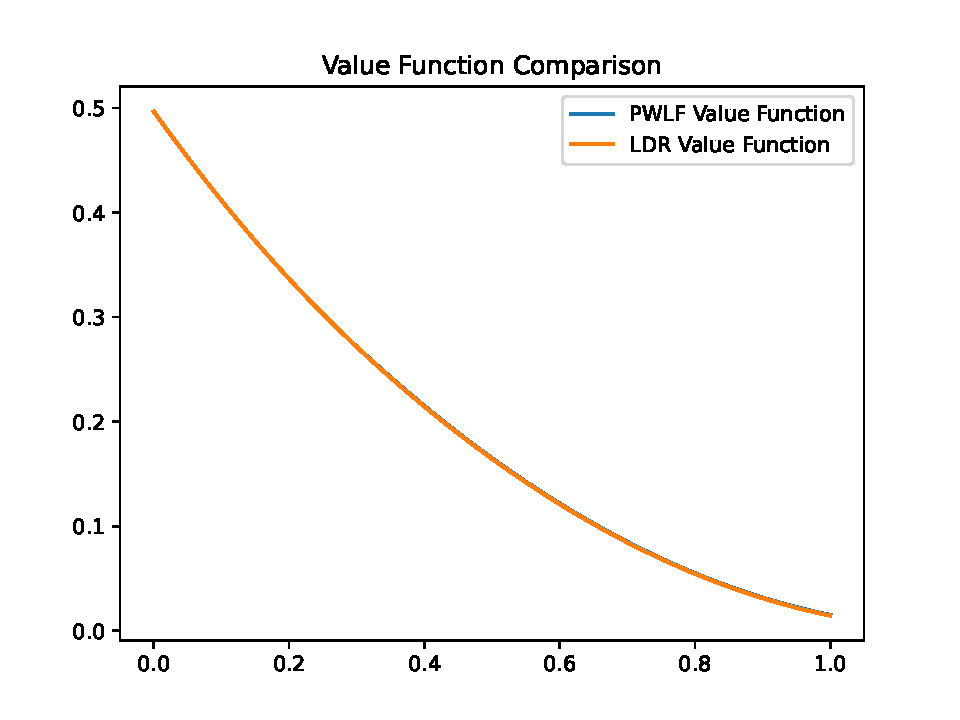
\includegraphics[height=0.8\textheight]{figures/1dtoy_value_function_comparison.pdf}
\end{frame}


\begin{frame}{Slightly more complex example}
  \begin{columns}
    \begin{column}{0.4\textwidth}
  \begin{itemize}
    \item Still one-dimensional;
    \item 24 stages, several thermal plants;
    \item Triangular uncertainty distribution;
    \item 20 breakpoints for the decision rules.
  \end{itemize}
    \end{column}
    \begin{column}{0.6\textwidth}
      \uncover<2->{
      \centering \includegraphics<-2>[height=0.8\textheight]{figures/1d_cost_scatter.pdf}
      \centering \includegraphics<3>[height=0.8\textheight]{figures/1d_cost_hist.pdf}
      }
    \end{column}
  \end{columns}
\end{frame}

\begin{frame}{Slightly more complex example}
  \centering 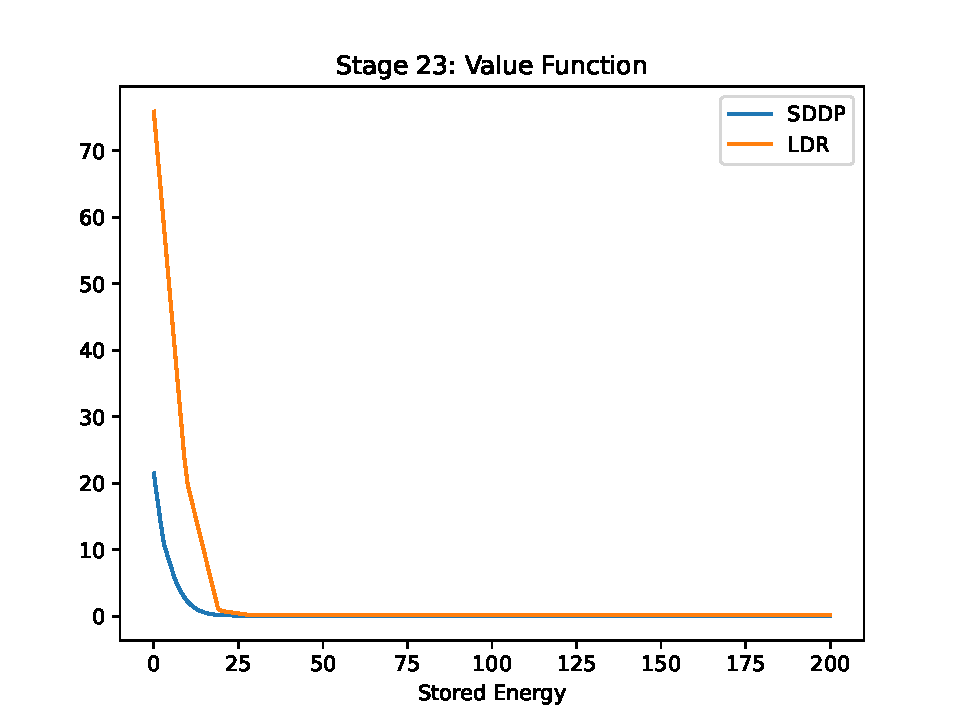
\includegraphics[width=0.45\textwidth]{figures/1d_vf_23.pdf} 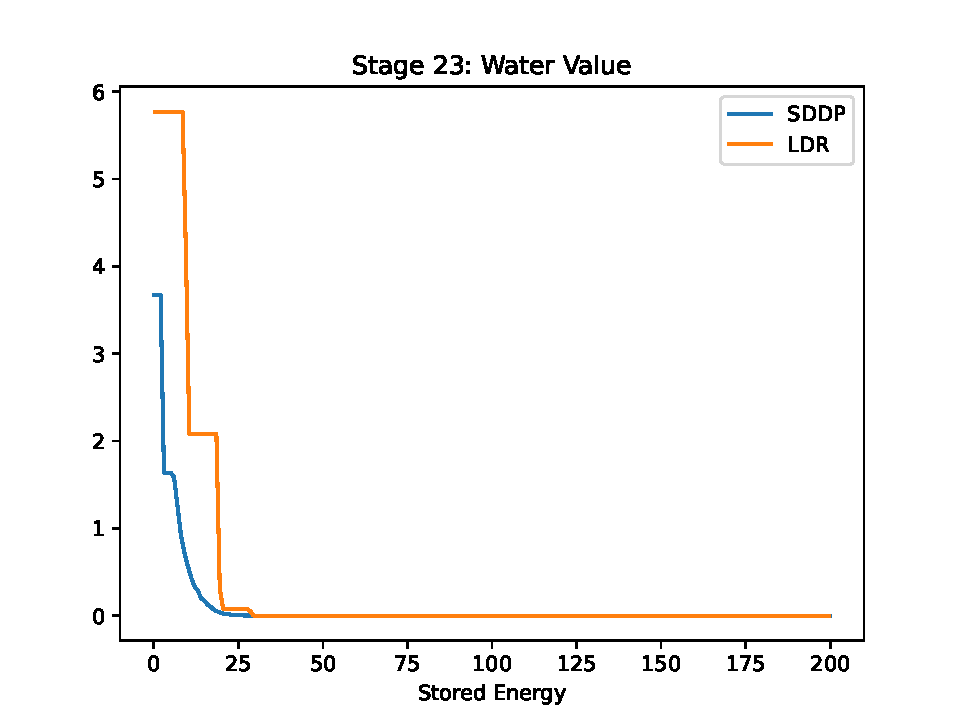
\includegraphics[width=0.45\textwidth]{figures/1d_water_value_23.pdf}
\end{frame}

\begin{frame}{Slightly more complex example}
  \centering 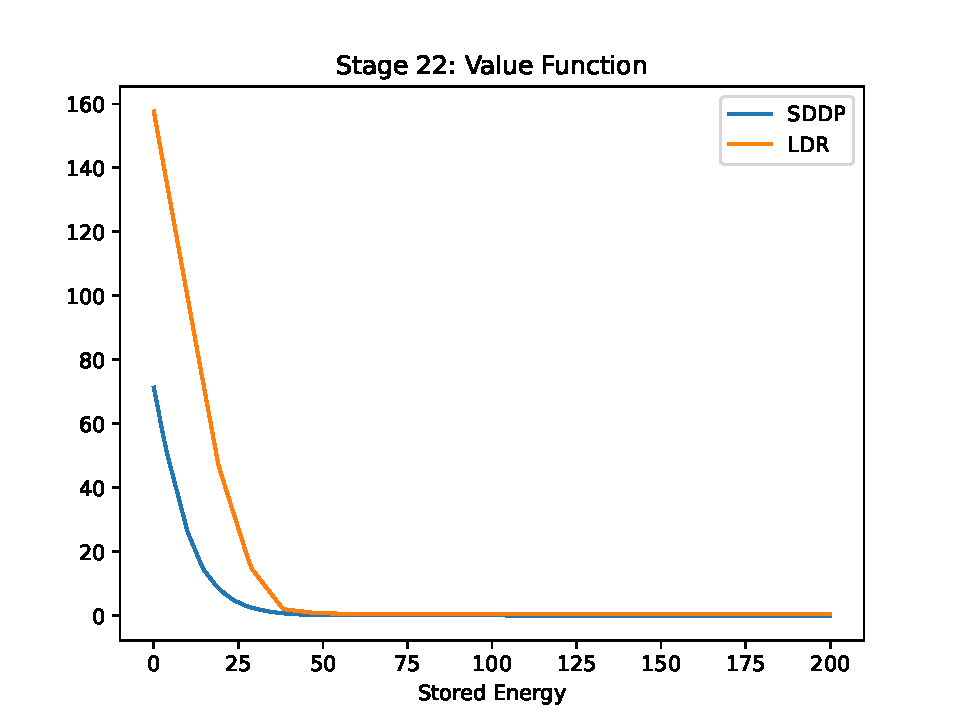
\includegraphics[width=0.45\textwidth]{figures/1d_vf_22.pdf} 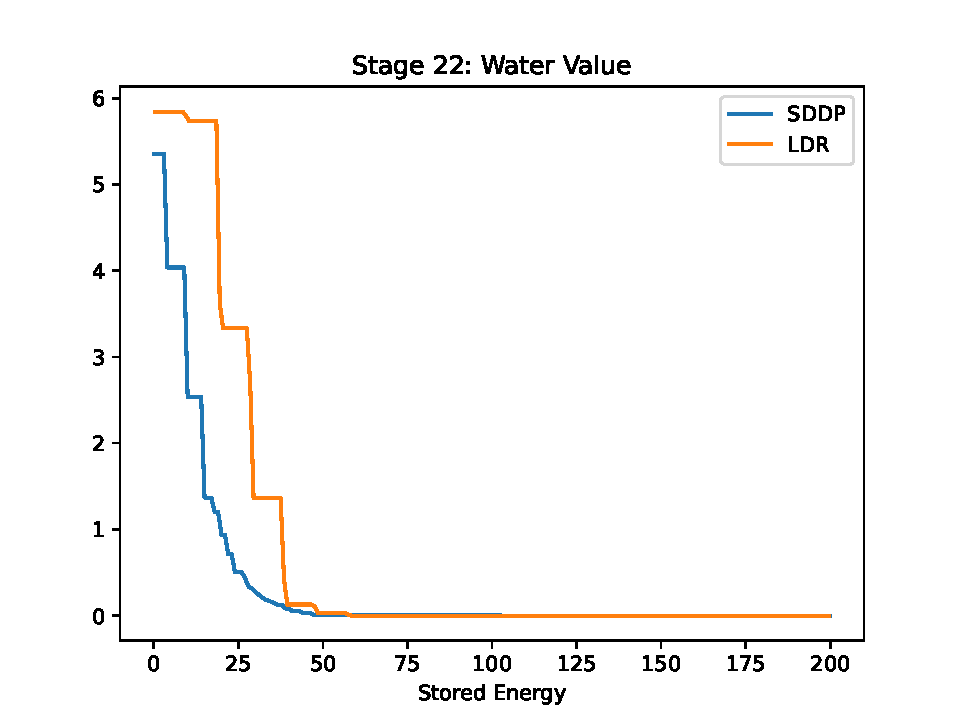
\includegraphics[width=0.45\textwidth]{figures/1d_water_value_22.pdf}
\end{frame}

\begin{frame}{Slightly more complex example}
  \centering 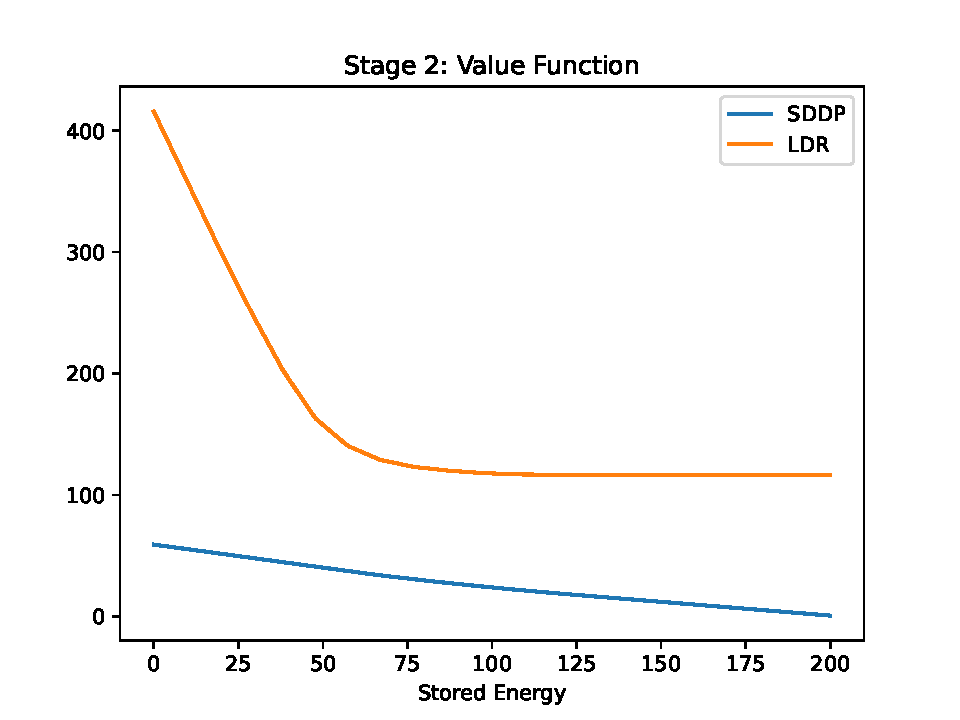
\includegraphics[width=0.45\textwidth]{figures/1d_vf_2.pdf} 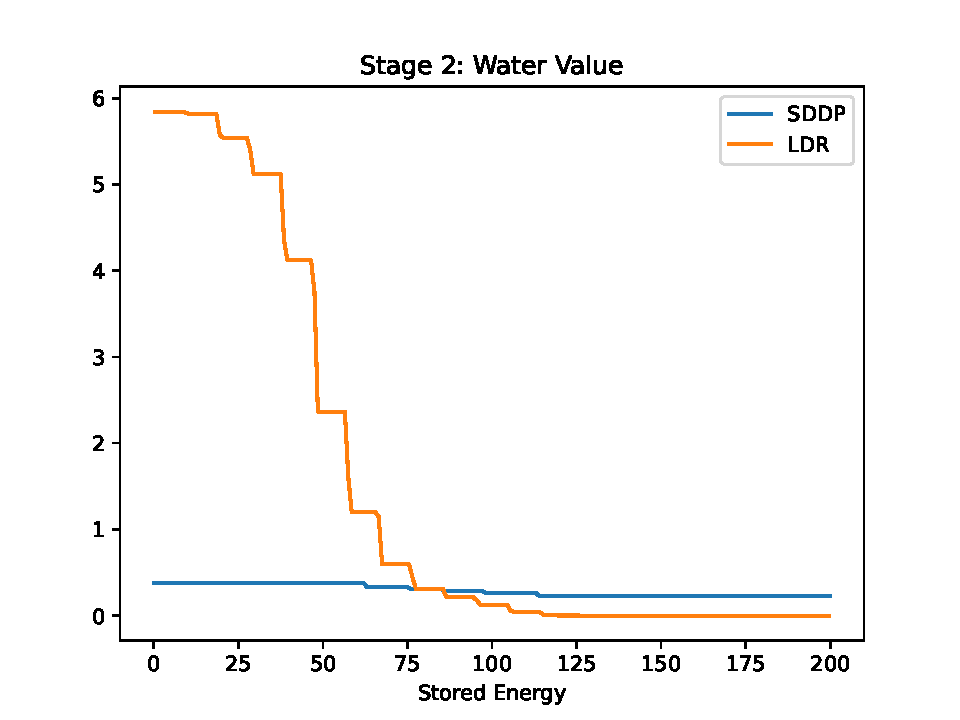
\includegraphics[width=0.45\textwidth]{figures/1d_water_value_2.pdf}
\end{frame}


\begin{frame}{Next steps}
  \emph{Multistage} decision rules:
  \begin{itemize}
    \item Generalize \alertt{FirstStage} to accommodate decisions $x_t$ which can only depend on \emph{observed} uncertainties $\xi_1, \ldots, \xi_t$;
    \item Will benefit from \alert{correlated uncertainties} to model more complex processes.
  \end{itemize}
  \pause\medskip

  \emph{Performance}:
  \begin{itemize}
    \item Speed-up \emph{model building} for larger problems (ongoing);
    \item \emph{Auto-tune breakpoints} (number and position);
    \item Adaptive \emph{state} distribution.
  \end{itemize}
\end{frame}

\setbeamertemplate{headline}{}
\begin{frame}
  \begin{columns}
    \begin{column}{0.5\textwidth}
      \centering
      \LARGE GitHub Package

      
\includegraphics[width=0.8\textwidth]{figures/ldrgit.pdf}
    \end{column}
    \begin{column}{0.5\textwidth}
      \centering
      \LARGE Documentation

      
\includegraphics[width=0.8\textwidth]{../Hydro25/figures/ldrdoc.pdf}
    \end{column}
  \end{columns}

  \centering
  \Huge Questions?
\end{frame}


\end{document}


% vim:set spelllang=en:
